\documentclass[tikz, border=3mm]{standalone}
\usepackage{tikz}
\usetikzlibrary{shapes.geometric, arrows, positioning, fit, calc}
\usepackage{fontspec}
\setmainfont{Times New Roman}
\begin{document}
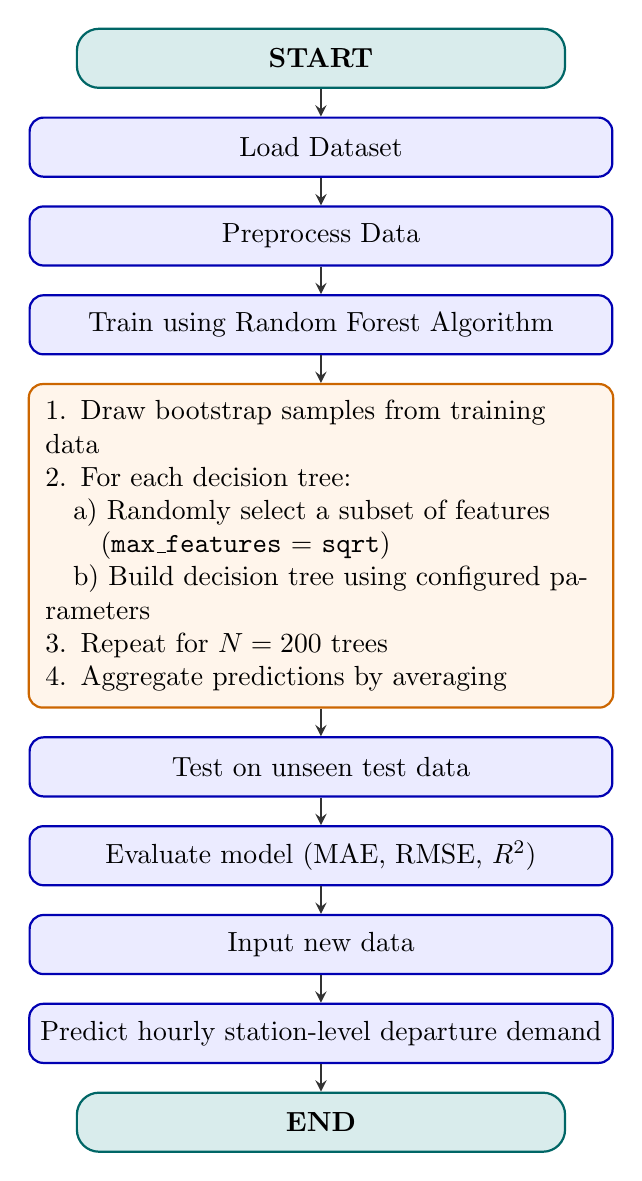
\begin{tikzpicture}[
    node distance=0.35cm,
    startstop/.style={rectangle, rounded corners=8pt, minimum width=6.2cm, minimum height=0.75cm, align=center, draw=teal!80!black, thick, fill=teal!15, font=\rmfamily\bfseries\normalsize, inner sep=4pt},
    proc/.style={rectangle, rounded corners=5pt, minimum width=7.4cm, minimum height=0.75cm, align=center, draw=blue!70!black, thick, fill=blue!8, font=\rmfamily\normalsize, inner sep=4pt},
    bigproc/.style={rectangle, rounded corners=5pt, minimum width=7.4cm, align=left, draw=orange!80!black, thick, fill=orange!8, font=\rmfamily\normalsize, text width=7.0cm, inner sep=6pt},
    arrow/.style={thick, ->, >=stealth, draw=black!80}
]

\node (start) [startstop] {START};
\node (load) [proc, below=0.35cm of start] {Load Dataset};
\node (prep) [proc, below=0.35cm of load] {Preprocess Data};
\node (train) [proc, below=0.35cm of prep] {Train using Random Forest Algorithm};
\node (bootstrap) [bigproc, below=0.35cm of train] {
1. Draw bootstrap samples from training data\\
2. For each decision tree:\\
\quad a) Randomly select a subset of features\\
\quad\quad (\texttt{max\_features} = \texttt{sqrt})\\
\quad b) Build decision tree using configured parameters\\
3. Repeat for $N = 200$ trees\\
4. Aggregate predictions by averaging
};
\node (test) [proc, below=0.35cm of bootstrap] {Test on unseen test data};
\node (eval) [proc, below=0.35cm of test] {Evaluate model (MAE, RMSE, $R^2$)};
\node (input) [proc, below=0.35cm of eval] {Input new data};
\node (predict) [proc, below=0.35cm of input] {Predict hourly station-level departure demand};
\node (end) [startstop, below=0.35cm of predict] {END};

\draw [arrow] (start) -- (load);
\draw [arrow] (load) -- (prep);
\draw [arrow] (prep) -- (train);
\draw [arrow] (train) -- (bootstrap);
\draw [arrow] (bootstrap) -- (test);
\draw [arrow] (test) -- (eval);
\draw [arrow] (eval) -- (input);
\draw [arrow] (input) -- (predict);
\draw [arrow] (predict) -- (end);

\end{tikzpicture}
\end{document}
